% !TeX root = L5_02_27_2026.tex

\documentclass{beamer}
\usepackage{svg}
\usepackage{tikz}
\usepackage{tabularx}
\usepackage{amsmath,mathtools,amssymb,amsfonts}
\usepackage{pgfplots}

\pgfplotsset{compat=1.18}

\title{Multiple Linear Regression}
\logo{\includesvg[width=1.2cm]{../NBU}}
\author[Bhaya, A.G.]{Bhaya, A.G.\\University of North Bengal\\ \href{mailto:angubh.io@gmail.com}{ananya.gb@nbu.ac.in}}
\date{February 27, 2026}

\usetikzlibrary{arrows.meta, positioning}
\usetheme{Berkeley}
\usecolortheme{default}

\begin{document}
    \begin{frame}
        \titlepage
    \end{frame}

    \begin{frame}{Contents}
        \tableofcontents
    \end{frame}

    \section{Introduction}
    \begin{frame}{Introduction}
        In the previous lecture, we studied about single variable linear regression. It involved a single variable, with two parameters, needed to find an estimate \(\hat{y}=c_0x+c_1\).

        Now we are going to study about multivariate regression (or multiple linear regression). In this type of regression, we find an estimate involving multiple variables (say \(n\)), with multiple parameters (\(n+1\)). 
    \end{frame}

    \begin{frame}{Example}
        Let us consider an example. We want to build a regressional model, which estimates the price of a house (\(y\)), based on three factors, area (\(x_1\)), number of bathrooms (\(x_2\)), and number of bedrooms (\(x_3\)).

        \begin{table}
            \centering
            \begin{tabularx}{0.75\textwidth}{|X|X|X|X|}
                \hline
                \(y\) (in \$) & \(x_1\) & \(x_2\) & \(x_3\)\\
                \hline
                220 & 1600 & 2.5 & 3\\
                180 & 1400 & 1.5 & 3\\
                350 & 2100 & 3.5 & 4\\
                \(\vdots\) & \(\vdots\) & \(\vdots\) & \(\vdots\)\\
                500 & 2400 & 4 & 5\\
                \hline
            \end{tabularx}
            \caption{House prices data.}
        \end{table}
    \end{frame}

    \begin{frame}
        \begin{figure}[h!]
            \centering
            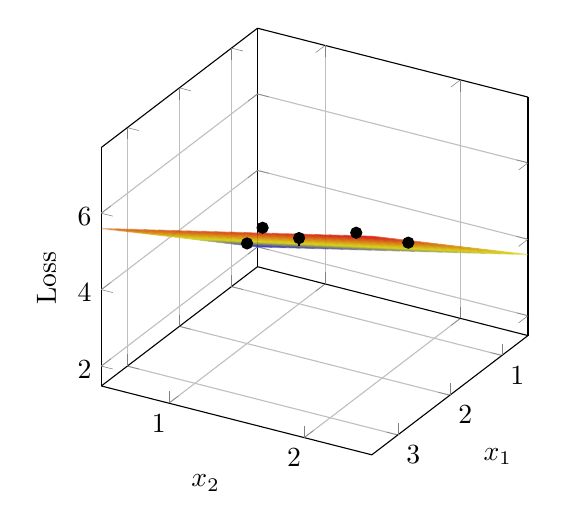
\begin{tikzpicture}
                \begin{axis}[
                    view={120}{30},
                    width=7cm,
                    height=7cm,
                    xlabel={$x_1$},
                    ylabel={$x_2$},
                    zlabel={Loss},
                    grid=major,
                ]

                % --- Scattered points ---
                \addplot3[
                    only marks,
                    mark=*,
                    mark size=2pt,
                ]
                coordinates {
                (1,1,3.2)
                (2,1,4.1)
                (1.5,2,4.5)
                (2.5,2,5.8)
                (3,1.5,6.0)
                };

                % --- Best fit plane ---
                \addplot3[
                    surf,
                    opacity=0.4,
                    domain=0.5:3.5,
                    y domain=0.5:2.5,
                    samples=20,
                ]
                {1 + 1.2*x + 0.8*y};

                % --- Residual (loss direction lines) ---
                \addplot3[thick]
                coordinates {(1,1,3.2) (1,1,{1 + 1.2*1 + 0.8*1})};

                \addplot3[thick]
                coordinates {(2,1,4.1) (2,1,{1 + 1.2*2 + 0.8*1})};

                \addplot3[thick]
                coordinates {(1.5,2,4.5) (1.5,2,{1 + 1.2*1.5 + 0.8*2})};

                \end{axis}
                \end{tikzpicture}
                \caption{Representation of best-fit plane for the above example.}
        \end{figure}
    \end{frame}

    \section{Multiple Linear Regression}
    \begin{frame}{Multiple Linear Regression}
        \begin{block}{Multiple Linear Regression}
            \textbf{Multiple Linear Regression (MLR)} is a statistical method used to model the relationship between one dependent variable, adn two or more independent variables by fitting a linear equation to observed data. It assumes response variable depends linearly on several predictors.
        \end{block}      
        
    \end{frame}

    \subsection{Mathematical Interpretation of MLR}
    \begin{frame}{Mathematical Interpretation of MLR}
        For \(p\) variables, estimation (\(\hat{y}\)) using multiple linear regression, is defined by,

        \begin{equation}
            \hat{y}=\beta_0+\beta_1x_1+\beta_2x_2+\hdots+\beta_px_p+\epsilon
        \end{equation}

        where,

        \begin{itemize}
            \item \(y\) is the dependent (response) variable
            \item \(x_1,x_2,\hdots,x_p\) are independent (predictor) variables
            \item \(\beta_0\) is the intereceptor (bias term)
            \item \(\beta_1, \beta_2,\hdots,\beta_p\) are the regression coefficients
            \item \(\epsilon\) is the random error term
        \end{itemize}

    \end{frame}

    \begin{frame}
        In terms of linear algebra, for a dataset with \(m\times n\) dimensions, we define,

        \begin{align*}
            X&=\left[\begin{array}{c c c c}
                1 & x_{11} & \hdots & x_{1n}\\
                1 & x_{21} & \hdots & x_{2n}\\
                1 & x_{31} & \hdots & x_{3n}\\
                \vdots & \vdots & \hdots & \vdots\\
                1 & x_{m1} & \hdots & x_{mn}
            \end{array}\right],
            \beta=\left[\begin{array}{c}
                \beta_0\\
                \beta_1\\
                \beta_2\\
                \vdots\\
                \beta_n
            \end{array}\right]\textnormal{and, }
            y&=\left[\begin{array}{c}
                y_1\\
                y_2\\
                y_3\\
                \vdots\\
                y_m
            \end{array}\right]
        \end{align*}

        Hence the equation for MLR can be represented by,

        \begin{equation}
            \boxed{y=X\beta}
        \end{equation}
    \end{frame}

    \section{Least Squares Estimate in MLR}
    \begin{frame}{Least Squares Estimate}{in Multiple Linear Regression}
        The loss function of MLR is represented by,
            \begin{equation}\label{eq:3}
                L(\beta)=(X\beta-y)^T(X\beta-y)
            \end{equation}

        The gradient of the loss function (equation \eqref{eq:3}) is given by,
        \begin{equation}\label{eq:4}
            \nabla L(\beta)=2X^T(X\beta-y)
        \end{equation}

        Upon minimizing equation \eqref{eq:4}, we get our parameter vector \(\beta\), as shown below,
        \begin{align}
            X^TX\beta&=X^Ty\nonumber\\
            \Rightarrow \beta&=(X^TX)^{-1}X^Ty
        \end{align}

        \begin{block}{Note}
            \(X^TX\) is the Hessian matrix, which is positive semi-definite.
        \end{block}
    \end{frame}

    \begin{frame}
        \begin{alertblock}{Practice Set}
            Solve the practice set of questions for this lecture titled: \textbf{L5\_02\_27\_2026\_Practice\_Set}.
        \end{alertblock}
    \end{frame}

\end{document}